\section*{Лекция 14 (19.05)}

\subsection{Задачи о цепной лиинии}



\tikzset{every picture/.style={line width=0.75pt}} %set default line width to 0.75pt        

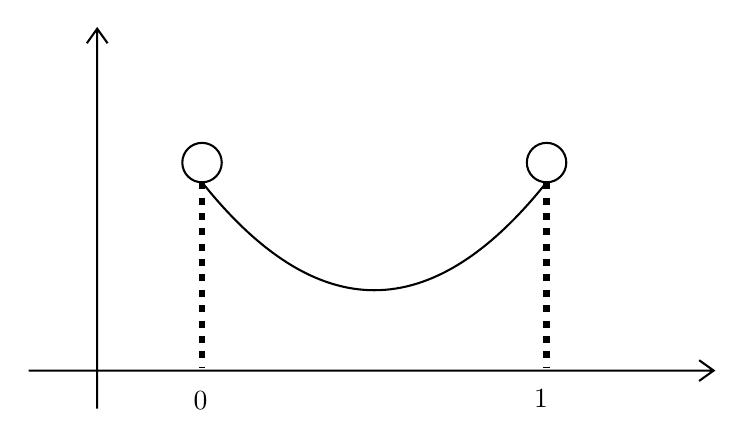
\begin{tikzpicture}[x=0.75pt,y=0.75pt,yscale=-1,xscale=1]
%uncomment if require: \path (0,300); %set diagram left start at 0, and has height of 300

%Shape: Circle [id:dp6470834655648232] 
\draw   (131,132.5) .. controls (131,127.25) and (135.25,123) .. (140.5,123) .. controls (145.75,123) and (150,127.25) .. (150,132.5) .. controls (150,137.75) and (145.75,142) .. (140.5,142) .. controls (135.25,142) and (131,137.75) .. (131,132.5) -- cycle ;
%Shape: Circle [id:dp4667573510460582] 
\draw   (297,132.5) .. controls (297,127.25) and (301.25,123) .. (306.5,123) .. controls (311.75,123) and (316,127.25) .. (316,132.5) .. controls (316,137.75) and (311.75,142) .. (306.5,142) .. controls (301.25,142) and (297,137.75) .. (297,132.5) -- cycle ;
%Shape: Parabola [id:dp9673957977293743] 
\draw   (140.5,142) .. controls (195.83,211.33) and (251.17,211.33) .. (306.5,142) ;
%Shape: Axis 2D [id:dp7229525297219248] 
\draw  (57,232.7) -- (387,232.7)(90,68) -- (90,251) (380,227.7) -- (387,232.7) -- (380,237.7) (85,75) -- (90,68) -- (95,75)  ;
%Straight Lines [id:da6982113442625548] 
\draw [line width=2.25]  [dash pattern={on 2.53pt off 3.02pt}]  (140.5,142) -- (140.5,231) ;
%Straight Lines [id:da32744740902138914] 
\draw [line width=2.25]  [dash pattern={on 2.53pt off 3.02pt}]  (306.5,142) -- (306.5,231) ;

% Text Node
\draw (135,241.4) node [anchor=north west][inner sep=0.75pt]    {$0$};
% Text Node
\draw (299,240.4) node [anchor=north west][inner sep=0.75pt]    {$1$};


\end{tikzpicture}

Потенциальная энергия:

\[
    \Pi(f) = \int_0^1 f(x)\sqrt{1 + (f'(x)) ^ 2} dx \to \min
\]

Т.к. $\Pi = mgh$, а в нашем случае $h = f(x)$, а за вес мы тут берем просто длину цепочки.

Ограничение на длину:

\[
    \Phi(f) = \int_0^1 \sqrt{1 + (f'(x))^2} dx - l = 0
\]


Метод множителей Лагранжа говорит, что
$f$ --- условный локальный минимум 
$\hence \exists \lambda : \forall h$ 
допустимого приращения : $h(0) = h(1) = 0$ 

\[
    \partial_h (\Pi - \lambda \Phi)(f) = 0  \quad \quad (1)
\]

\[
    (\Pi - \lambda \Phi)(f) = \int_0^1 F(x, f(x), f'(x)) dx
\]

Тогда: $F(x, u, v) = (u - \lambda) \sqrt{1 + v ^ 2}$

(1) $\hence$ Ур. Эйлера-Лагранжа

Заметим, что $F$ не зависит от x, то есть $F = F(u, v)$

\[
    (\star) = \partial_2 F - \frac{d}{dx} \partial_3 F = 0 \hence F - f' \partial_3 F = ci
\]

Это мы просто угадали, давайте проверим:

\[
    F - f' \partial_3 F = c \quad \bigg | \frac{d}{dx}
\]

Посмотрим на дифференциал: $\frac d {dx} F = \partial_2 F \cdot f' + \partial_3 F \cdot f''$ и $\frac d {dx} (- f' \cdot \partial_3 F) = -f'' \cdot \partial_3 F - f' \frac d {dx} (\partial_3 F)$

\[
    \partial_2 F f' + \partial_3 F \cdot f'' - f'' \cdot \partial_3 F - f' \frac{d}{dx}(\partial_3 F) = 0 \Leftrightarrow
\]


\[
    \Leftrightarrow \partial_2 F f' - f' \frac{d}{dx}(\partial_3 F) = 0
\]

\[
    \Rightarrow (\star) = (f(x) - \lambda) \sqrt{1 + (f'(x)) ^ 2} - f'(x) \cdot (f(x) - \lambda) \cdot \frac{f'(x)}{\sqrt{1 + (f'(x)) ^ 2}} = c \Rightarrow
\]

\[
    \Rightarrow \frac{1}{\sqrt{1 + (f')^2}} = \frac{c}{f - \lambda} \Rightarrow \frac{1}{1 + (f')^2} = (\frac{c}{f - \lambda}) ^ 2 \Rightarrow 1 + (f') ^ 2 = \left(\frac{f - \lambda}{c}\right) ^ 2 \Rightarrow
\]

\[
    \Rightarrow f' = \sqrt{\frac{(f -  \lambda)  ^ 2 - c ^ 2}{c ^ 2}} \Rightarrow \frac{f'}{\sqrt{(f - \lambda) ^ 2 - c ^ 2}} = \frac{1}{c}
\]

\[
    \Rightarrow \int \frac{f'}{\sqrt{(f - \lambda) ^ 2 - c ^ 2}} dx = \int \frac{1}{c} dx \Rightarrow
\]

\[
    \Rightarrow \int \frac {df} {\sqrt{(f - \lambda)^2 - c^2}} = \int \frac 1 c dx
\]

\[
    \log(f - \lambda + \sqrt{(f - \lambda) ^ 2 - c ^ 2}) = \frac{1}{c} x + c_1
\]


$f(x)$ --- какой-то гиперпобилеский косинус

$f(x) - \lambda = ch(\frac{1}{c} x + c_1)$


\subsection{Задача о поверхности вращения наименьшей площади}



\tikzset{every picture/.style={line width=0.75pt}} %set default line width to 0.75pt        

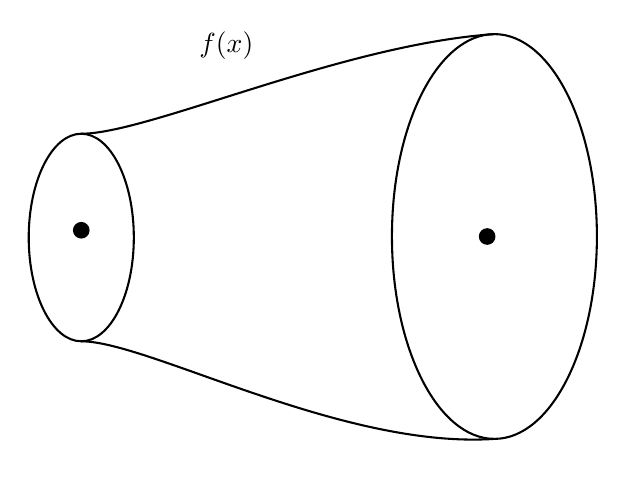
\begin{tikzpicture}[x=0.75pt,y=0.75pt,yscale=-1,xscale=1]
%uncomment if require: \path (0,300); %set diagram left start at 0, and has height of 300

%Shape: Ellipse [id:dp08320508738413235] 
\draw   (100.25,142) .. controls (100.25,114.39) and (111.59,92) .. (125.57,92) .. controls (139.55,92) and (150.89,114.39) .. (150.89,142) .. controls (150.89,169.61) and (139.55,192) .. (125.57,192) .. controls (111.59,192) and (100.25,169.61) .. (100.25,142) -- cycle ;
%Shape: Ellipse [id:dp826690931291277] 
\draw   (275.25,141.51) .. controls (275.25,87.66) and (297.36,44) .. (324.63,44) .. controls (351.89,44) and (374,87.66) .. (374,141.51) .. controls (374,195.36) and (351.89,239.02) .. (324.63,239.02) .. controls (297.36,239.02) and (275.25,195.36) .. (275.25,141.51) -- cycle ;
%Curve Lines [id:da45633667729745897] 
\draw    (125.57,92) .. controls (158,92) and (251,49) .. (324.63,44) ;
%Curve Lines [id:da6723971457827435] 
\draw    (125.57,192) .. controls (158,192) and (251,244.02) .. (324.63,239.02) ;
%Shape: Circle [id:dp4260812331849331] 
\draw  [fill={rgb, 255:red, 0; green, 0; blue, 0 }  ,fill opacity=1 ] (122.07,138.5) .. controls (122.07,136.57) and (123.63,135) .. (125.57,135) .. controls (127.5,135) and (129.07,136.57) .. (129.07,138.5) .. controls (129.07,140.43) and (127.5,142) .. (125.57,142) .. controls (123.63,142) and (122.07,140.43) .. (122.07,138.5) -- cycle ;
%Shape: Circle [id:dp6733942956964831] 
\draw  [fill={rgb, 255:red, 0; green, 0; blue, 0 }  ,fill opacity=1 ] (317.63,141.51) .. controls (317.63,139.58) and (319.19,138.01) .. (321.13,138.01) .. controls (323.06,138.01) and (324.63,139.58) .. (324.63,141.51) .. controls (324.63,143.44) and (323.06,145.01) .. (321.13,145.01) .. controls (319.19,145.01) and (317.63,143.44) .. (317.63,141.51) -- cycle ;

% Text Node
\draw (181,41.4) node [anchor=north west][inner sep=0.75pt]    {$f( x)$};


\end{tikzpicture}

Площадь поверхности:

\[
    S(f) = \int_0^1 2 \Pi f(x) \sqrt{1 + (f'(x)) ^ 2} dx
\]


\[
    \partial_2 F - \frac{d}{dx} \partial_3 F = 0 \hence f \text{ --- гиперпоболический косинус}
\]

\subsection{\textit{Последний} :) Сжимающие отображения и решения дифференциальных уравнений }


\begin{theorem}
    $(X, \rho)$ --- полное метрическое пространство, $U : X \to X$ --- сжимающее, т.е. $\exists \gamma < 1 : \forall x_1, x_2 \in X, \rho(U(x_1), U(x_2)) \leqslant \gamma \rho (x_1, x_2) \hence \exists ! x_* : U(x_*) = x_*$
\end{theorem}

\begin{proof}
    $x_0 \in X, x_1 = U(x_0), ..., x_{n + 1} = U(x_n)$

    \[
        \rho(x_{n + 1}, x_n) \leqslant \gamma \rho (x_n, x_{n - 1}) \leqslant \gamma ^ 2 \rho (x_{n - 1}, x_{n - 2}) \leqslant ... \leqslant \gamma ^ n \rho(x_1, x_0)
    \]

    $m > n:$

    \[
        \rho(x_m, x_n) \leqslant \rho(x_m, x_{m - 1}) + ... + \rho(x_{n + 1}, x_n) \leqslant (\gamma ^ {m - 1} + \gamma^{m - 2} + ... + \gamma ^ n) \rho(x_1, x_0) \leqslant \frac{\gamma ^ n}{1 - \gamma} \rho(x_1, x_0)
    \]

    $m > n > N \hence \rho(x_m, x_n) \leqslant C \cdot \gamma ^ N \hence \{ x_n \}$ --- фунд. $\hence \exists$ предел $\lim x_n = x_*$

    Доказательство единственности:

    $x_*, x_*' \hence \rho(U(x_*), U(x_*')) < \rho(x_*, x_*')$
\end{proof}

\follow $(X, \rho)$ --- полное метрическое пространство, $U : X \to X$, но $\exists n : U ^ n$ --- сжимающее отображение $\hence \exists! $ неподвижная точка для $U$


\begin{proof}
    Для $U ^ n$ есть сжимающая точка $x_*$




    \tikzset{every picture/.style={line width=0.75pt}} %set default line width to 0.75pt        

    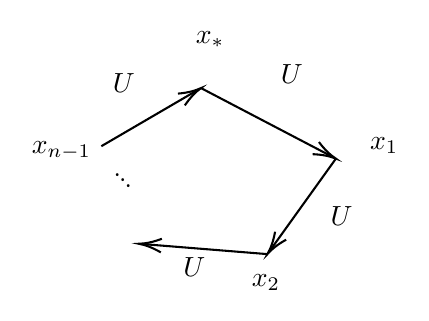
\begin{tikzpicture}[x=0.75pt,y=0.75pt,yscale=-1,xscale=1]
    %uncomment if require: \path (0,300); %set diagram left start at 0, and has height of 300
    
    %Straight Lines [id:da452542765364476] 
    \draw    (255,133) -- (318.23,166.07) ;
    \draw [shift={(320,167)}, rotate = 207.61] [color={rgb, 255:red, 0; green, 0; blue, 0 }  ][line width=0.75]    (10.93,-3.29) .. controls (6.95,-1.4) and (3.31,-0.3) .. (0,0) .. controls (3.31,0.3) and (6.95,1.4) .. (10.93,3.29)   ;
    %Straight Lines [id:da8941010038622086] 
    \draw    (320,167) -- (288.17,211.37) ;
    \draw [shift={(287,213)}, rotate = 305.66] [color={rgb, 255:red, 0; green, 0; blue, 0 }  ][line width=0.75]    (10.93,-3.29) .. controls (6.95,-1.4) and (3.31,-0.3) .. (0,0) .. controls (3.31,0.3) and (6.95,1.4) .. (10.93,3.29)   ;
    %Straight Lines [id:da519003009540322] 
    \draw    (287,213) -- (226.99,208.16) ;
    \draw [shift={(225,208)}, rotate = 4.61] [color={rgb, 255:red, 0; green, 0; blue, 0 }  ][line width=0.75]    (10.93,-3.29) .. controls (6.95,-1.4) and (3.31,-0.3) .. (0,0) .. controls (3.31,0.3) and (6.95,1.4) .. (10.93,3.29)   ;
    %Straight Lines [id:da7190351834005099] 
    \draw    (207,161) -- (253.27,134.01) ;
    \draw [shift={(255,133)}, rotate = 149.74] [color={rgb, 255:red, 0; green, 0; blue, 0 }  ][line width=0.75]    (10.93,-3.29) .. controls (6.95,-1.4) and (3.31,-0.3) .. (0,0) .. controls (3.31,0.3) and (6.95,1.4) .. (10.93,3.29)   ;
    
    % Text Node
    \draw (292,120.4) node [anchor=north west][inner sep=0.75pt]    {$U$};
    % Text Node
    \draw (251,104.4) node [anchor=north west][inner sep=0.75pt]    {$x_{*}$};
    % Text Node
    \draw (335,155.4) node [anchor=north west][inner sep=0.75pt]    {$x_{1}$};
    % Text Node
    \draw (278,221.4) node [anchor=north west][inner sep=0.75pt]    {$x_{2}$};
    % Text Node
    \draw (316,188.4) node [anchor=north west][inner sep=0.75pt]    {$U$};
    % Text Node
    \draw (213.79,170.77) node [anchor=north west][inner sep=0.75pt]  [rotate=-45,xslant=-0.07] [align=left] {...};
    % Text Node
    \draw (172,157.4) node [anchor=north west][inner sep=0.75pt]    {$x_{n-1}$};
    % Text Node
    \draw (245,213.4) node [anchor=north west][inner sep=0.75pt]    {$U$};
    % Text Node
    \draw (211,124.4) node [anchor=north west][inner sep=0.75pt]    {$U$};
    
    
    \end{tikzpicture}

$\hence U ^ n$ имеет > 1  неподвижной точки
\end{proof}

\subsubsection*{Дифференциальные уравнения}

Однородное дифференциальное уравнение первого порядка $f'(x) = F(f(x), x), F(f', f, x) = 0$

Рассмотрим уравнения:

$f'(x) = A(x) f(x) + B(x), f \in C^1[a, b], f(a) = 0$

\begin{enumerate}
    \item Переделать в интегральное уравнение 
    \[
        f(x) = \int_a^x A(t)f(t)+B(t) dt
    \]

    Хотим найти неподвижные точки $U$

    \[
        U : f \to \int_a ^ x A(t) f(t) + B(t) dt
    \]

    $X = \{ f \in C[a, b] , f(a) = 0 \}$ --- полное метрическое пространство

    \[
        \norm{Uf_1 - Uf_2} = \max_{x \in [a, b]} \abs{\int_a^x A(t)f_1(t) - A(t) f_2(t) dt} \leqslant (b - a) \max \abs{A} \cdot \norm{f_1 - f_2} \leqslant M \cdot (b - a) \cdot \norm{f_1 - f_2}
    \]

    Поэтому отображение $U$ не сжимающее.

    \[
        \norm{U ^ n f_1 - U^n f_2} = ?
    \]

Сначала разберемся без сдвига на $B$.

    \[
        U_0 f(x) = \int_a ^ x A(t) f(t) dt
    \]

    \[
        U_0 ^ n f(x) =  \int_a^x  ... \int_a^{t_3} A(t_2) (\int_0^{t_2} A(t_1) (\int_0^{t_1} A(t) f(t) dt ) dt_1) dt_2 ... dt_{n - 1}
    \]

    \[
        \norm{U_0 ^ n (f_1 - f_2) } \leqslant \norm{f_1 - f_2} \cdot M ^ n \cdot \max_{x \in [a,b]} \underbrace{\abs{ \int_a^x \int_a^{t_{n - 1}} ... \int_a^{t_1} dt dt_1 ... dt_{n-1}}}_{\frac{(x - a) ^ n}{n !}} \leqslant \norm{f_1 - f_2} \cdot \frac{M ^ n \cdot (b - a) ^ n}{n !}
    \]

    $\hence \exists n : \frac{M ^ n (b -a)}{n !} < 1$

    $
        U ^ n (f_1) - U^n(f_2) = U_0 ^ n (f_1) - U_0 ^ n (f_2) \hence U ^ n
    $ сжимающее

    $\hence \exists! f_* : f_*(x) = \int_a^x A(t) f_*(t) + B(t) dt, f_*(a) = 0, f_* \in C[a, b]$.
    
    Но если $A, B \in C[a, b] \hence f_* \in C^1 [a, b]$
\end{enumerate}


